\input{../slides-common/preambule}

\pdsetup{
   lf = {\cursopequeno},
   rf = {Interconexão}, palette = {\palette}, randomdots={false},
   cf = {\theslide}
}


%opening
\title{\cursogrande\\ \vspace{1cm}{Interconexão entre componentes de um computador}}

\begin{document}
   \maketitle[randomdots={false}]
   
   \begin{slide}{Agenda}
      \tableofcontents[content=sections]
   \end{slide}
%%%%%%%%%%%%%%%%%%%%%%%%%%%%%%%%%%%%%%%%%%%%%%%%%%%%%%
\section[slide=true]{Estruturas de interconexão}
\begin{slide}{Estruturas de interconexão}
	\twocolumn{
	\begin{itemize}
		\item Computador: conjunto de módulos.
		\item Estrutura de interconexão: comunicação entre módulos
		\item Entradas e saídas típicas:
			\begin{itemize}
				\item Memória\\
					\begin{center}
						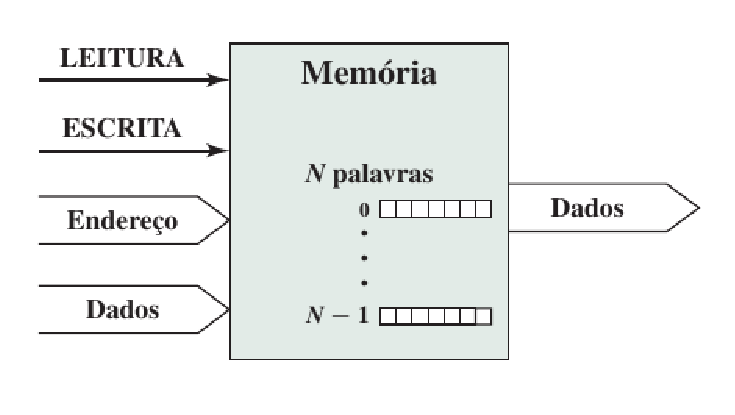
\includegraphics[width = 0.8\textwidth]{figs/3-15a}
					\end{center}
			\end{itemize}
	\end{itemize}
	}{
	\begin{itemize}
		\item Entradas e saídas típicas:
			\begin{itemize}
				\item Dispositivos de E/S\\
					\begin{center}
						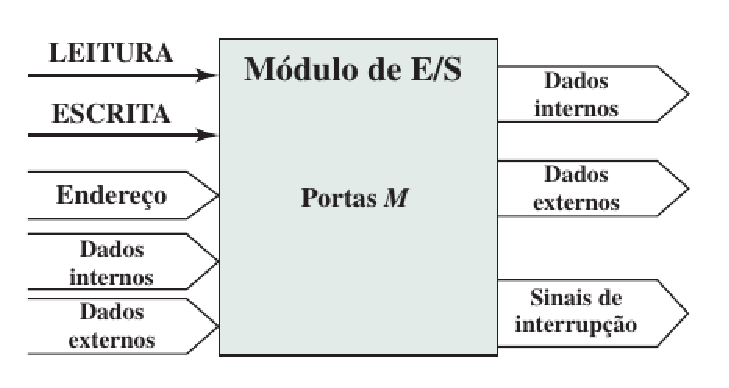
\includegraphics[width = 0.8\textwidth]{figs/3-15b}
					\end{center}
				\item Processador\\
					\begin{center}
						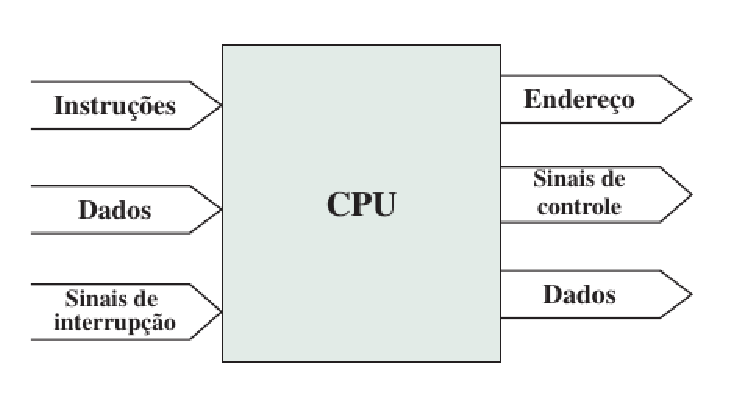
\includegraphics[width = 0.8\textwidth]{figs/3-15c}
					\end{center}
			\end{itemize}
	\end{itemize}}
\end{slide}
\section[slide=true]{Interconexão por barramento}
\begin{slide}{Interconexão por barramento}
	\begin{itemize}
		\item Barramento: caminho de comunicação que conecta dois ou mais dispositivos.
		\item O barramento é compartilhado:
			\begin{itemize}
				\item Sinais transmitidos por um dispositivo ficam disponíveis para todos os outros dispositivos conectados ao barramento.
				\item Somente um dispositivo pode transmitir por vez.
			\end{itemize}
		\item O barramento é composto, em geral, de múltiplos caminhos de comunicação ou linhas:
			\begin{itemize}
				\item Em cada linha são transmitidos sinais representando 0 ou 1.
				\item Transmissão de bits: em série (uma linha) ou em paralelo (múltiplas linhas).
				\item Tipos de linhas:
					\begin{itemize}
						\item Dados: o conjunto forma o \emph{barramento de dados}.
						\item Endereços: o conjunto forma o \emph{barramento de endereços}.
						\item Controle: o conjunto forma o \emph{barramento de controle}.
					\end{itemize}
			\end{itemize}
	\end{itemize}
\end{slide}

\begin{slide}{Barramento de controle}
	Linhas típicas de controle:
	\begin{itemize}
		\item Escrita em memória
		\item Leitura em memória
		\item Escrita em porta de E/S
		\item Leitura em porta de E/S
		\item Reconhecimento (ACK) de transferência
		\item Requisição de barramento
		\item Concessão de barramento
		\item Requisição de interrupção
		\item Reconhecimento de interrupção
		\item Clock
		\item Reset
	\end{itemize}
\end{slide}

\begin{slide}{Ilustração de um barramento}
   \centering
   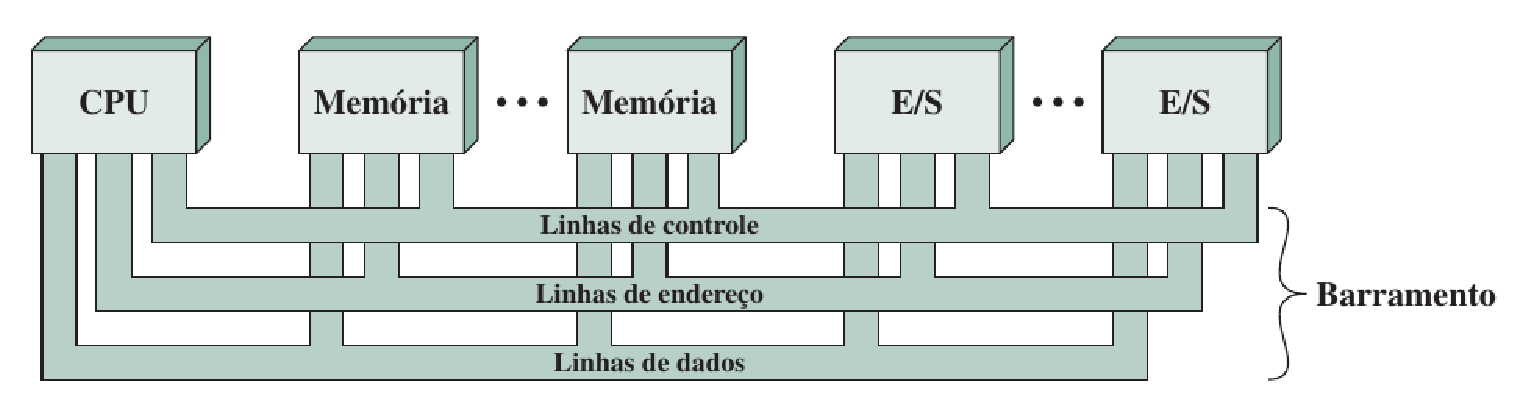
\includegraphics[width=0.95\textwidth]{figs/3-16}
\end{slide}

\section[slide=true]{Interconexão ponto a ponto}
\begin{slide}{Interconexão ponto a ponto}
\begin{itemize}
   \item Aumento de frequência em barramentos:
	   \begin{itemize}
		   \item Sincronização e arbitração cada vez mais difícil.
	   \end{itemize}
   \item Processadores multicore:
	   \begin{itemize}
		   \item Problemas com latência, taxa de bits e escalabilidade em barramentos compartilhados
	   \end{itemize}
   \item QuickPath Interconnect (QPI, Intel 2008):
	   \begin{itemize}
		   \item Conexões diretas múltiplas
		   \item Arquitetura de protocolo em camadas: parecido com TCP/IP
		   \item Transferência de dados em pacotes
	   \end{itemize}
   \end{itemize}
\end{slide}

\begin{slide}{Configuração multicore usando QPI}
	\centering
	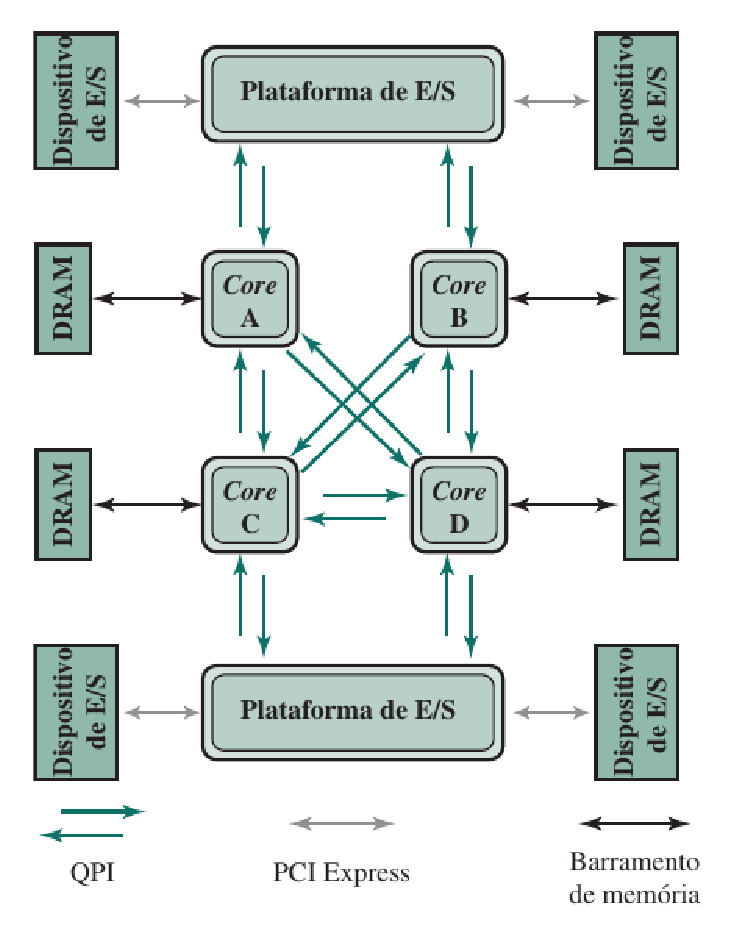
\includegraphics[height=0.8\textheight]{figs/3-17}
\end{slide}

\begin{slide}{Arquitetura QPI}
	Camadas da arquitetura QPI:
	\begin{itemize}
		\item Física: circuitos e conexões, Phit (physical unit, 20 bits).
		\item Ligação: transmissão confiável e controle de fluxo, Flit (flow control unit, 80 bits).
		\item Roteamento: estrutura de redirecionamento de pacotes (número inteiro de Flits).
		\item Protocolo: conjunto de regras para a troca de pacotes.
	\end{itemize}
   \centering
   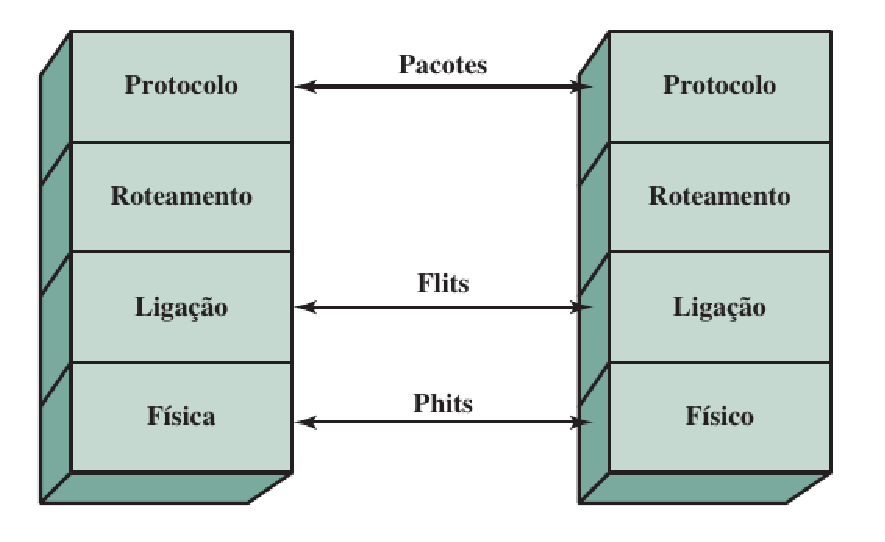
\includegraphics[width=0.6\textwidth]{figs/3-18}
\end{slide}

% redação em andamento
%\section[slide=true]{PCI Express}
%\begin{slide}{PCI Express}
%	\begin{itemize}
%		\item \textit{Peripheral Component Interconnect}
%		\item Barramento de grande largura de banda
%		\item Melhor desempenho para subsistemas de E/S de alta velocidade
%			\begin{itemize}
%				\item Adaptadores gráficos de vídeo
%				\item Controladoras de interface de rede
%				\item Controladores de disco
%			\end{itemize}
%		\item PCIe: nova versão da especificação PCI para atender às demandas de maior taxa de dados
%			\begin{itemize}
%				\item Esquema de interconexão ponto a ponto
%				\item Capacidade de suportar maiores taxas de dados
%				\item Trabalha com \textit{streams} de dados dependentes de tempo
%				\item Tratamento de dados por prioridade
%			\end{itemize}
%	\end{itemize}
%\end{slide}
%
%\begin{slide}{Arquitetura física}
%Exemplo de arquitetura física
%   \centering
%   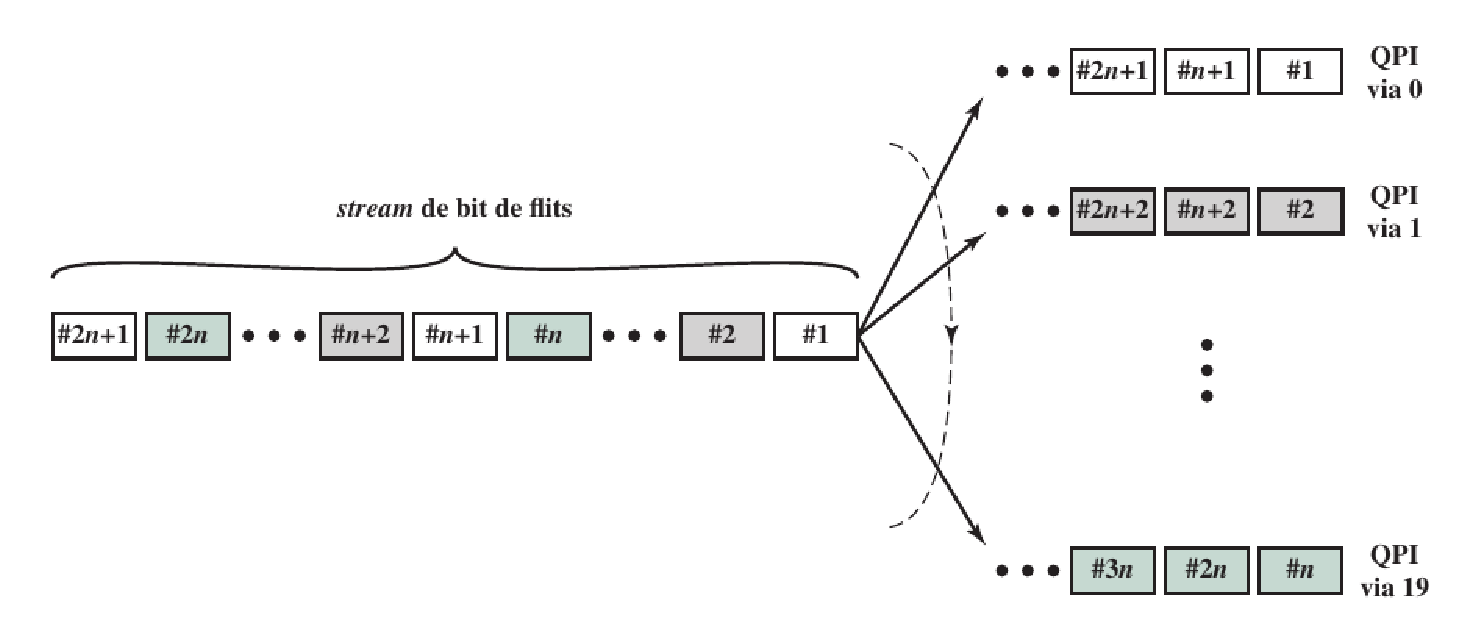
\includegraphics[width=0.8\textwidth]{figs/3-20}
%\end{slide}
%
%\begin{slide}{Arquitetura lógica}
%	Camadas da arquitetura de protocolo PCIe
%   \centering
%   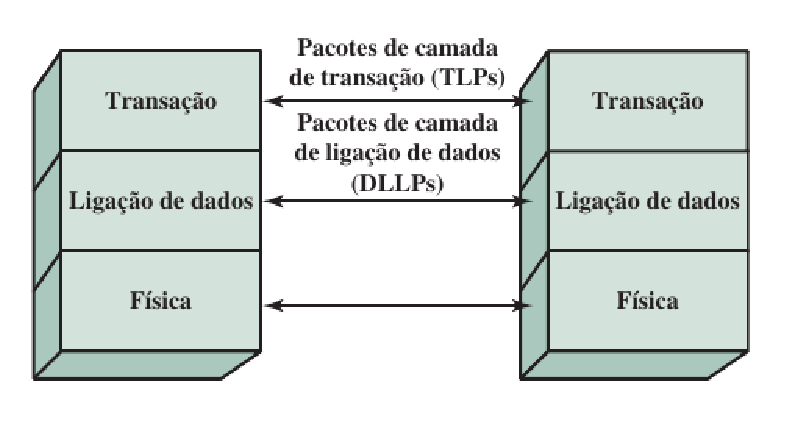
\includegraphics[width=0.8\textwidth]{figs/3-22}
%\end{slide}
%
%\begin{slide}{Camada física}
%	\begin{itemize}
%		\item Conexões reais e circuitos
%		\item Número de vias bidirecionais em uma porta: 1, 4, 6, 16, ou 32
%		\item Exemplo: porta PCIe de 4 vias
%			\centering
%			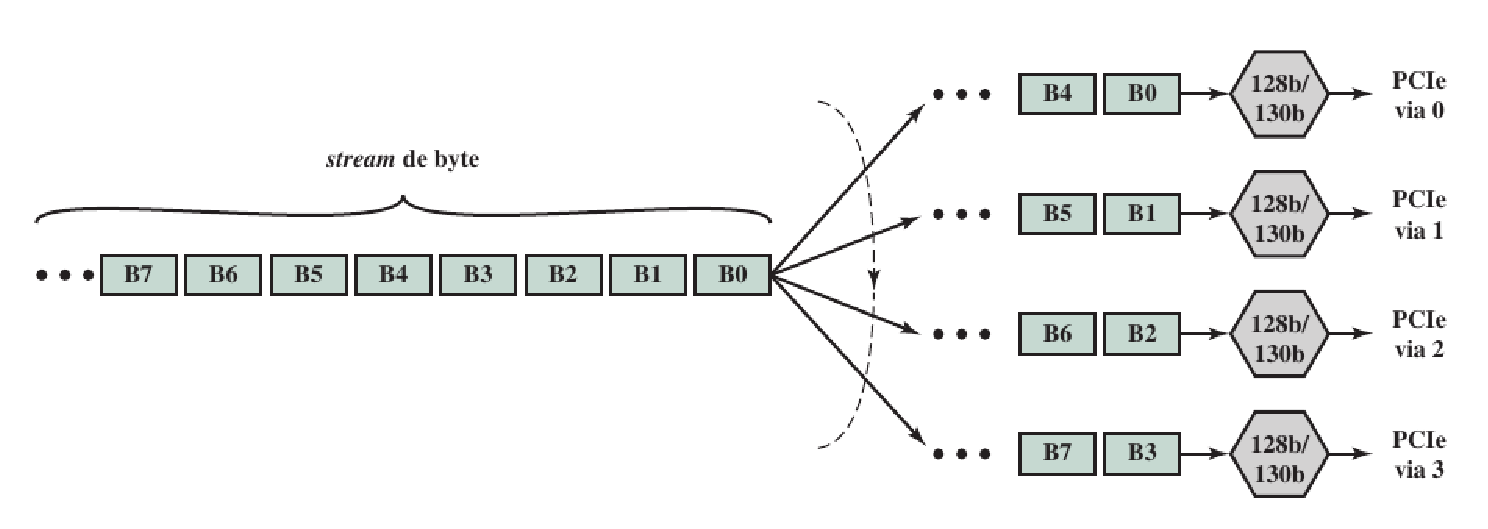
\includegraphics[width=0.9\textwidth]{figs/3-23}
%	\end{itemize}
%\end{slide}
%
%\begin{slide}{Camada de ligação de dados}
%	\begin{itemize}
%		\item \textit{Data link layer}
%		\item Transmissão de confiável
%		\item Controle de fluxo
%		\item Trabalha com pacotes (\textit{data link layer packets}, DLLP)
%	\end{itemize}
%\end{slide}
%
%\begin{slide}{Camada de transação}
%	\begin{itemize}
%		\item Pacote da camada de transação (\textit{transaction layer packets}, TLP)
%		\item Implementa mecanismos de transferênciade dados de armazenamento de carga
%		\item Gerencia o controle de fluxo de TLPs entre dois componentes de um link
%	\end{itemize}
%\end{slide}
\end{document}
